%%%% Input Codes %%%%   
% <mcode.sty> required for Matlab codes
% template for inserting codes:

% \lstset{numbers=left,numberstyle= \tiny}
% \lstinputlisting[firstline=6, lastline=15]{/Users/name/Desktop/FILENAME.M}

% or:

%\lstset{numbers=left,numberstyle= \tiny}
%\begin{lstlisting}[xleftmargin=2em,xrightmargin=2em,aboveskip=1em]
%clc; clear all; close all;
%\end{lstlisting}

Start by \href{http://www.econ.yale.edu/smith/paper15.pdf}{Krusell and Smith (2006)}, and learning about heterogeneous agent models (Wouter den Haan's \href{http://www.wouterdenhaan.com/numerical/introhetero.pdf}{introductory slides}. There is also a handbook chapter on solving and simulating models with heterogeneous agents by \href{http://www.wouterdenhaan.com/numerical/handbookhetero.pdf}{Algan et al (2010)}.) \\


\section{Basic Model Set up}

The key technical things for Heterogeneous Agent Models are distribution of agents, which relates to individual choices and aggregate variables is an {\color{red} infinite dimensional object}(many state variables). 

For every type $i$ agent we have the general formula of equilibrium: 
\[ 
E_t f(x^i_{t-1}, x^i_{t}, x^i_{t+1},u^i_{t},u^i_{t+1},x_{t-1}, x_{t}, x_{t+1},u_{t},u_{t+1})=0, 
\]


where, $x$ is endogenous variables, $u$ denotes exogenous. 

And for aggregate and individual endogenous variables, we have: 
\[
x_t \equiv \int \gamma (x_t^i)d_t (i)di \quad \text{with } \int d_t (i)di = 1 
\]

Law of motion of the density function (share of each type $i$ agent): 
\[ d_t (\cdot) = \mathcal{P}(d_{t-1}(\cdot), u_t)\]

\subsection{Krusell\&Smith Model}

Individual endogenous variables: $x^i_t = \{c^i_t,a^i_t\}$;\\

Aggregate endogenous variables: $x_t = W_t,R_t,K_t,Y_t$;\\

Exogenous variables: idiosyncratic shocks $s^i_t$ and TFP shocks $z_t$.\\

HH foc: 
\begin{align}
\begin{split}
(c^i_t)^{-\sigma} = \beta E_t R_{t+1}(c^i_{t+1})^{-\sigma} \quad \text{if } a^i_t > a_{min} \\
(c^i_t)^{-\sigma} > \beta E_t R_{t+1}(c^i_{t+1})^{-\sigma} \quad \text{if } a^i_t = a_{min} \\
c^i_t + a^i_t = s^i_t W_t + a^i_{t-1} R_{t-1}
\end{split}\label{hhfoc}
\end{align}

by Firm Maximization problem: 
\begin{align}
\begin{split}
W_t = (1-\alpha)Y_t/L_{t} \\
R_t = \alpha Y_t/K_{t-1} + (1- \delta)
\end{split}
\end{align} 


And market clearing condition for assets: $\int a^i_t d_t (i)di = K_t$\\

Above is a way of describing the models generally. In {\color{red} PS1 and PS2}, we solve KS model by using \textbf{Krusell-Smith Algorithm with conventional VFI}, in the Literature later on, some extensions from Krusell-Smith Algorithm are described. In this Final Project, I want to learn an advanced method for solving DSGE models, which is frequently used in recent researches, the projection and perturbation methods. Specifically, I'm going to use Reiter method on solving KS model.\\

\section{Literature Review}\label{secLiter}

Start from Incomplete market model, with market frictions that cannot insure idiosyncratic risks, in our model, with only one asset but two risks. Krusell and Smith (1998) \cite{krusell1998income} developed such type of DSGE models which I described above, which characterizes both idiosyncratic risk and aggregate risks, and with heterogeneous agents.

To deal with such quantitative models, one strand of literature approximates the cross-sectional distribution using a parametric family, like Algan, Allais and Den Haan (2008)\cite{algan2008solving} in which they solve for the dynamics of the distribution using a globally accurate projection technique.\\

Another strand of literature uses a mix of globally accurate and locally accurate approximations to solve for the dynamics of heterogeneous agent models like Reiter (2009)\cite{reiter2009solving}, he solves the individual problem with a projection method, and approximates the law of motion of aggregate variables and the distribution with a perturbation method.\\

However, approximates the distribution with a fine histogram, which requires many parameters to achieve acceptable accuracy. This limits Reiter (2009)\cite{reiter2009solving} approach to problems which have a low-dimensional individual state space because the size of the histogram grows exponentially in the number of individual states. More advanced things have been done by Winberry, Thomas (2018)\cite{winberry2018method}, where he approximates the distribution with a flexible parametric family, reducing its dimensionality to a finite set of endogenous parameters, and solve for the dynamics of these endogenous parameters by perturbation. This part of work can be found in  \href{http://faculty.chicagobooth.edu/thomas.winberry/research/index.html}{Winberry's website}\footnote{Thomas also provide codes for Benchmark RBC model with Firm Heterogeneity}

\section{Different Solution Methods}
\subsection{Krusell and Smith Algorithm}

We've already encountered the KS algorithm for solving HA DSGE model. Den Haan, Wouter (2010)\cite{den2010comparison} make very deep analysis about different algorithm on solving KS models. for KS algorithm, please see \href{https://github.com/davidrpugh/pyeconomics/wiki/Krusell-Smith-Algorithm}{Krusell Smith Algorithm} for more details

\subsection{Projection and Perturbation: Reiter Method}

For projection (or collocation) method, it uses the 'global' behavior of the functional equation to approximate solution, which requires finding zeros of non-linear equations\footnote{a disadvantage is time-consuming of iterative methods of doing this}, and can easily adapt to situations the policy rule is not continuous or simply non-differentiable (i.e., occasionally binding and zero lower bound). And for perturbation method, which uses Taylor series expansion (computed using implicit function theorem) to approximate the model solution, which can implement procedure using non-iterative methods (much more faster) but as we've encountered in Part\_A of our Quant Macro Session, the Taylor approximation or even Chebyshev approximation does not work when there are important non-differentiability such as zero lower bound or occasionally binding. 

Thankfully, in K\&S model, we don't impose non-differentiable constraints, thus, 1st order perturbation is enough to capture the properties.  

Now, we only {\color{red} discretized individual state space into grids}, and also the density function such that $\sum_{i=1}^{N} d^i_t = 1$ which is like discretization the continuous distribution with ``histograms''. And then, we could approximate individual policy function using a projection method:

\[ 
x^i_t \approx \tilde{g}(x^i_{t-1},u^i_t, \theta_t) \quad \text{for } x^i_t \equiv g(x^i_{t-1}, u^i_t, x_{t-1},u_t,d_{t-1}), 
\]

where $\theta_t$ is the vector of coefficients. 

\subsubsection*{Step 1: Solve for SS under General Equilibrium}

By discretization, we can solve individual policy function $x^i_t \approx \tilde{g}(x^i_{t-1},u^i_t, \theta_t)$ with a projection method\footnote{Setting aggregate shocks to zero, guess SS of capital, then we can solve for policy function coefficients $\theta$}, and use this policy function to compute the stationary distribution of agents. Then, we check market clearing condition $K=\sum_{i=1}^{N} a^i d^i$, and update $K$ until convergence

Another thing worth to notice is that during computing the evolution of distribution, we need next period asset $a^i_{next}$, in previous PS, I use interpolation once (faster) but mostly straightly rely on the grids of assets. Here, I use approximation based on interpolation weights $W_{ij}$ since next period assets are separated among different types on the grids: 
\[
 W_{ij}=
 \begin{cases}
 1- \frac{a^i_{next} - a_j}{a_{j+1}-a_j} \quad &\text{if } a^i_{next} \in [a_j, a_{j+1}]\\ 
 \frac{a^i_{next} - a_{j-1}}{a_{j}-a_{j-1}} \quad &\text{if } a^i_{next} \in [a_{j-1}, a_{j}] \\
 0  \quad &\text{otherwise } 
 \end{cases}. 
\]

Up to now, we have girds, predetermined transition probabilities, and obtained individual policy function, we can compute the {\color{red} evolution of distribution}: 
\[ \mathcal{P}_{i'|i} = w_{ij} \times Prob(s'| s^i), \]

where distribution of agents evolves according to $d_t = \mathcal{P'} d_{t-1}$. 

Now, we check market clearing condition: $residuals \equiv K - \sum_{i=1}^{N}a^i d^i$

\medskip

\textbf{Recap PS1} about the selection on $\mathcal{P}_{i'|i}$, if we assume $H=2$ histories of agents are the same, then we have: 
\[ 
\mathcal{P}_{i'|i}=
\begin{bmatrix}
& UB & UG & EB & EG \\
UB & p_B & p_B & 0 & 0\\ 
UG & 0 & 0 & 1-p_G & 1-p_G\\
EB & 1-p_B & 1-p_B & 0 & 0\\
EG & 0 & 0 & p_G & p_G\\
\end{bmatrix}
\]

Then, Household problem in Equation \ref{hhfoc} becomes\footnote{for S state spaces power of H same-histories type of agents: $I = S^H$}: 

\begin{align}
\begin{split}
(c^i_t)^{-\sigma} = \beta R_t E_t \sum_{j=1}^I \mathcal{P}_{ji} (c^i_{t+1})^{-\sigma} \quad \text{if } a^i_t > a_{min} \\
c^i_t + a^i_t = s^i_t W_t + R_{t-1} \sum_{j=1}^I \mathcal{P}_{ji} a^j_{t-1} \frac{d^j_{t-1}}{d^i_t} \\
d^i_t = \sum_{j=1}^N \mathcal{P}_{ji} d^j_{t-1}
\end{split}
\end{align}

\subsubsection*{Step 2: compute 1st-order Perturbation to approximate the model system equations}

Using Perturbation method to approximate the individual equations (in Step 1), Law of motion for distribution, market clearing condition using Sims' GENSYS algorithm (obtained from the Internet)

For perturbation method, I use 1st-order Taylor expansion approximation, and during reading lectures notes from online sources, I notice that recently, scholars are using ``Automatic Differentiation'' to approximate, I try to include them, but I didn't use them.

\subsubsection*{Step 3: Solve the linearized system of equation }
Now, by ``histogram'' the density function, aggregate endogenous variable $x_t$ can be approximated  as $\tilde{x_t} = (\theta_t, x_t, d_t)$, and update by:
\[ \tilde{x}_t \equiv G_x \tilde{x}_{t-1} + G_u u_t\]



\subsection{Winberry's Algorithm}

\newpage


\section{Quantitative Performance of Reiter method}

In practice, I use the following files (/matlab/Reiter)for computing, there's two important steps need to notice, one is the Algorithm, which we first compute the general equilibrium steady states, and then compute dynamics; another one is when computing dynamics, we use 1st order perturbation, whose codes could be found on Internet: 

% Please add the following required packages to your document preamble:
% \usepackage{booktabs}
\begin{table}[]
\begin{tabular}{@{}cccc@{}}
\toprule
file name          & functions                                                                                                                              &         &                                                                                  \\ \midrule
menufun\_Reiter.m  & main file                                                                                                                              &         &                                                                                  \\
setup\_KS          & KS model parameters setup                                                                                                              & Step. 0 &                                                                                  \\
model\_stst.m      & compute SS given initial guess                                                                                                         & Step. 1 & \begin{tabular}[c]{@{}c@{}}require:\\ EulerResid.m\\ BuildTrans.m\end{tabular} \\
linear\_solution.m & \begin{tabular}[c]{@{}c@{}}supplementary file from Sims gensys \\ for computing dynamics\\ , using 1st order perturbation\end{tabular} & Step. 2 & \begin{tabular}[c]{@{}c@{}}require:\\ gensys.m \\ jacob.m\end{tabular}           \\
impresp\_sims.m    & compute IRF                                                                                                                            & Output  &                                                                                  \\ \bottomrule
\end{tabular}
\end{table}


The corresponding heterogeneous assets distribution among agents and the Impulse Response function with respect to shocks are attached in the following:

\begin{figure}[H]
\caption{Asset Distribution}
\hspace{-2.0cm}
\begin{center}
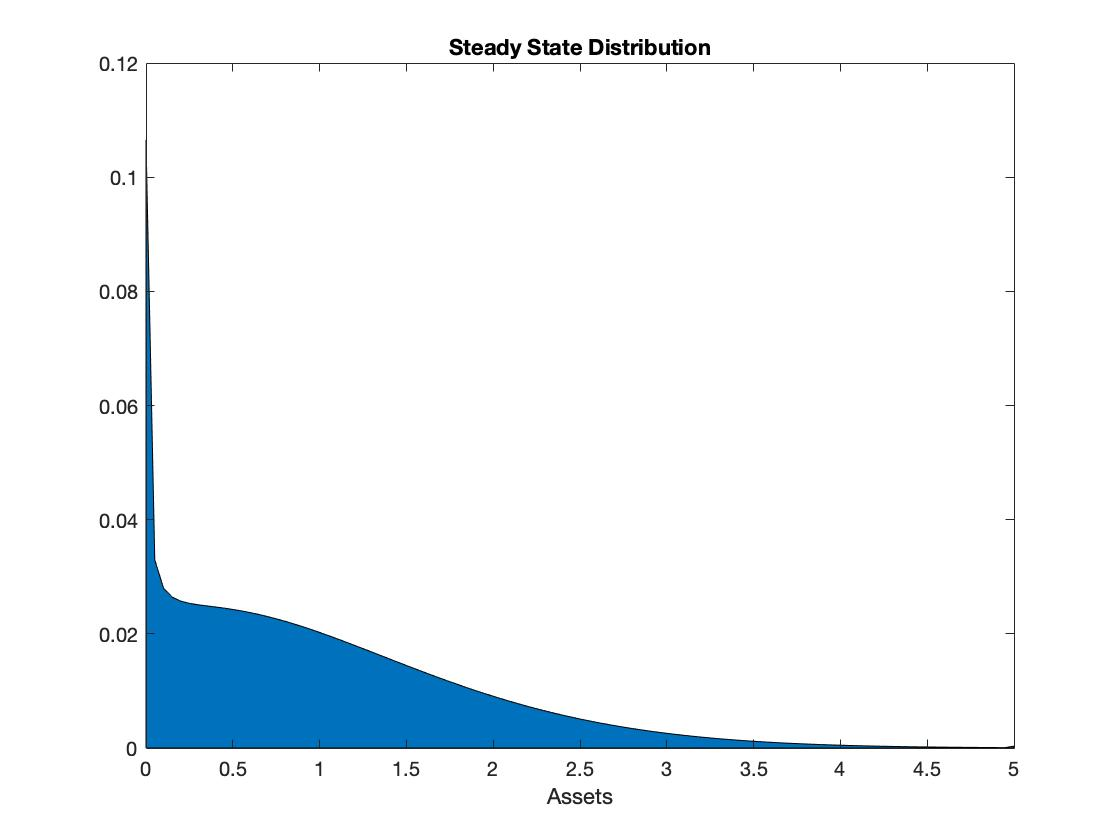
\includegraphics[angle=0,width=.67\textwidth]{img/1.jpg}
\end{center}
\end{figure}

\begin{figure}[H]
\caption{IRF by Reiter methods}
\hspace{-2.0cm}
\begin{center}
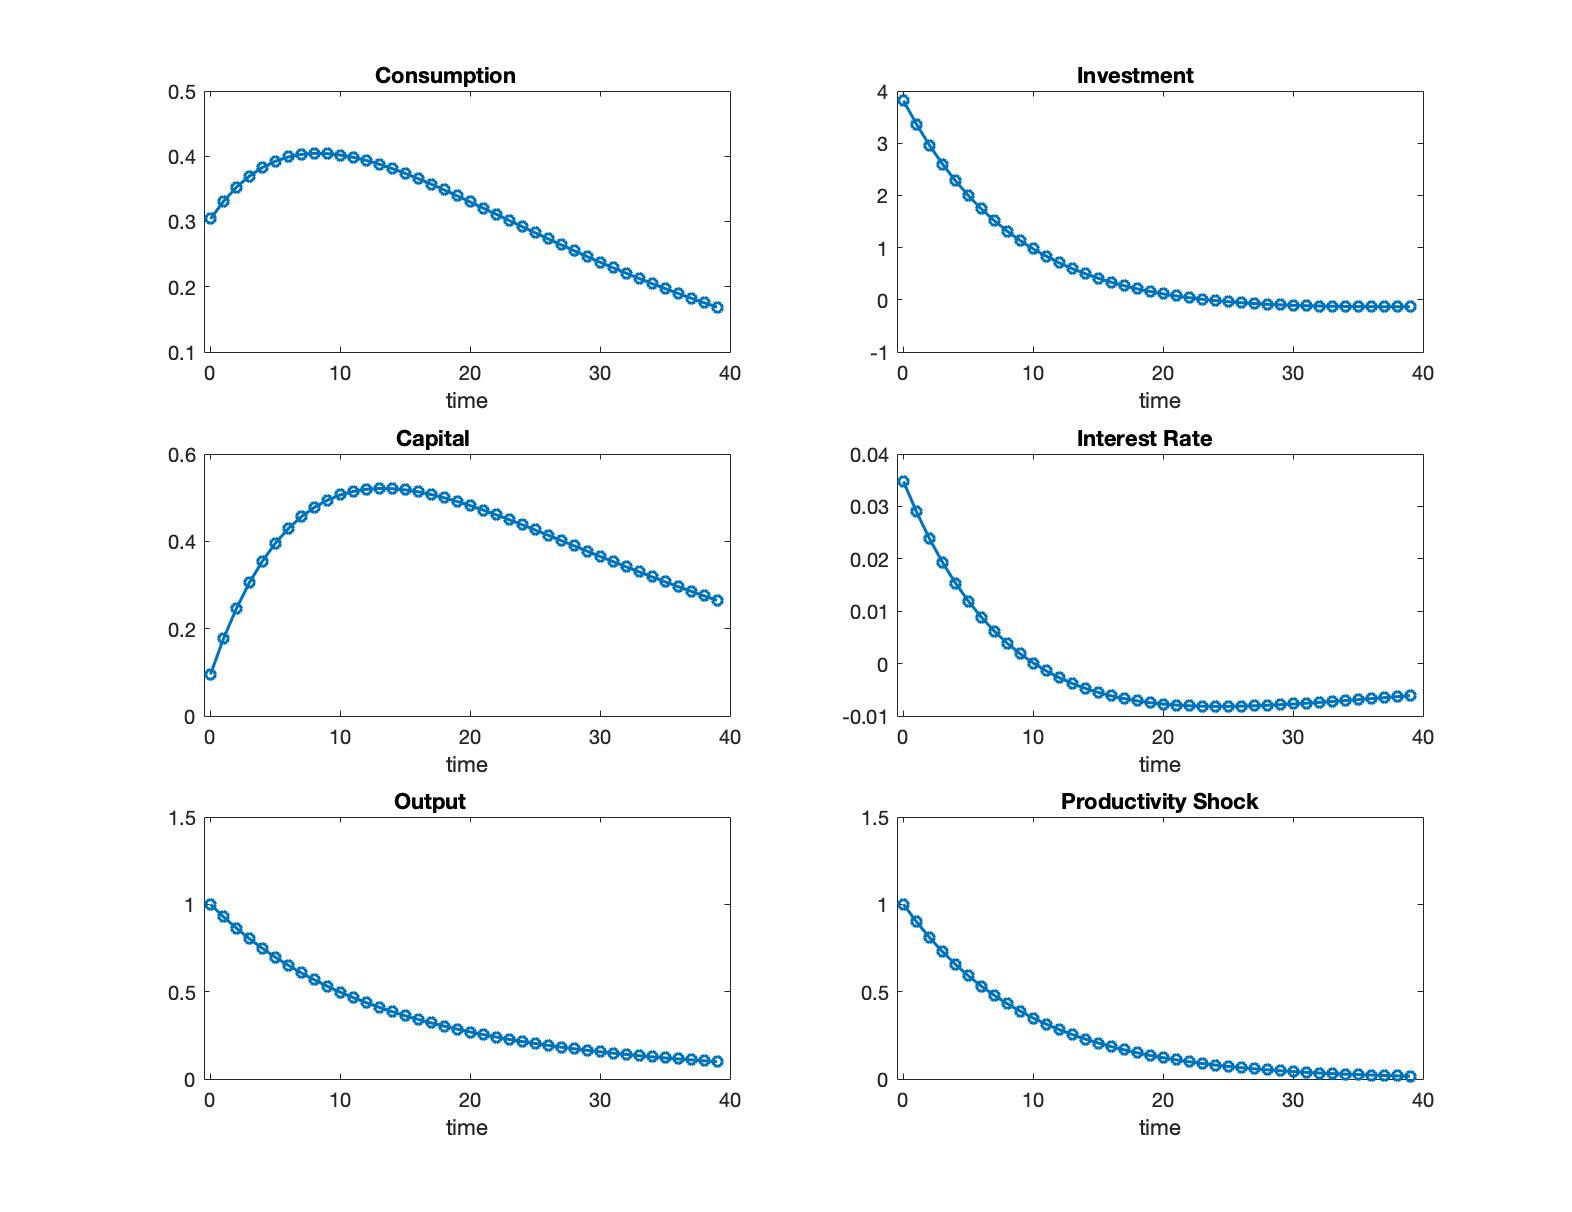
\includegraphics[angle=0,width=.67\textwidth]{img/2.jpg}
\end{center}
\end{figure}

Apart from the \href{http://www.wouterdenhaan.com/datasuite.htm}{corresponding websites} of Den Haan, Wouter (2010)\cite{den2010comparison}, which offers original Reiter codes, and others using different algorithms. I also list some resources about using Reiter Method to solve different set-up of DSGE models:

\begin{itemize}
\item \href{https://github.com/jeromematthewcelestine/hetagentsaggshocks}{Solves a simple model of firm investment with persistent aggregate and idiosyncratic productivity shocks}
\item \href{https://github.com/jeromematthewcelestine/hetagentsaggshocks}{Bayesian estimation of a heterogeneous agent DSGE model using the Reiter (2009) solution method}
\item \href{https://github.com/sebgraves/KS_and_Reiter}{Guide for solving the incomplete markets model using the methods of Krusell \& Smith (1998) and Reiter (2009)}
\end{itemize}

There's also a recent revised method on solving KS model by Thomas Winberry (2016), and I attach  the related files, in the future, I will learn about this methods.  